%% Copernicus Publications Manuscript Preparation Template for LaTeX Submissions
%% ---------------------------------
%% This template should be used for copernicus.cls
%% The class file and some style files are bundled in the Copernicus Latex Package, which can be downloaded from the different journal webpages.
%% For further assistance please contact Copernicus Publications at: production@copernicus.org
%% https://publications.copernicus.org/for_authors/manuscript_preparation.html


%% Please use the following documentclass and journal abbreviations for discussion papers and final revised papers.


%% 2-column papers and discussion papers
\documentclass[acp, manuscript]{copernicus}



%% Journal abbreviations (please use the same for discussion papers and final revised papers)

% Archives Animal Breeding (aab)
% Atmospheric Chemistry and Physics (acp)
% Advances in Geosciences (adgeo)
% Advances in Statistical Climatology, Meteorology and Oceanography (ascmo)
% Annales Geophysicae (angeo)
% ASTRA Proceedings (ap)
% Atmospheric Measurement Techniques (amt)
% Advances in Radio Science (ars)
% Advances in Science and Research (asr)
% Biogeosciences (bg)
% Climate of the Past (cp)
% Drinking Water Engineering and Science (dwes)
% Earth System Dynamics (esd)
% Earth Surface Dynamics (esurf)
% Earth System Science Data (essd)
% Fossil Record (fr)
% Geographica Helvetica (gh)
% Geoscientific Instrumentation, Methods and Data Systems (gi)
% Geoscientific Model Development (gmd)
% Geothermal Energy Science (gtes)
% Hydrology and Earth System Sciences (hess)
% History of Geo- and Space Sciences (hgss)
% Journal of Micropalaeontology (jm)
% Journal of Sensors and Sensor Systems (jsss)
% Mechanical Sciences (ms)
% Natural Hazards and Earth System Sciences (nhess)
% Nonlinear Processes in Geophysics (npg)
% Ocean Science (os)
% Proceedings of the International Association of Hydrological Sciences (piahs)
% Primate Biology (pb)
% Scientific Drilling (sd)
% SOIL (soil)
% Solid Earth (se)
% The Cryosphere (tc)
% Web Ecology (we)
% Wind Energy Science (wes)


%% \usepackage commands included in the copernicus.cls:
%\usepackage[german, english]{babel}
%\usepackage{tabularx}
%\usepackage{cancel}
%\usepackage{multirow}
%\usepackage{supertabular}
%\usepackage{algorithmic}
%\usepackage{algorithm}
%\usepackage{amsthm}
%\usepackage{float}
%\usepackage{subfig}
\usepackage{rotating}


\begin{document}

\title{Emissions of trace gases from Australian temperate forest fires: emission factors and dependence on modified combustion efficiency}


% \Author[affil]{given_name}{surname}

\Author[1]{Elise-Andr\'ee}{Gu\'erette}
\Author[1]{Clare}{Paton-Walsh}
\Author[1]{Maximilien}{Desservettaz}
\Author[2]{Thomas E.L}{Smith}
\Author[3]{Liubov}{Volkova}
\Author[3]{Christopher J.}{Weston}
\Author[4]{C.P. (Mick)}{Meyer}

\affil[1]{Centre for Atmospheric Chemistry, School of Chemistry, University of Wollongong, Wollongong, NSW, Australia}
\affil[2]{Department of Geography, King's College London, London, UK}
\affil[3]{School of Ecosystem and Forest Sciences, the University of Melbourne, Creswick, VIC, Australia}
\affil[4]{CSIRO Oceans and Atmosphere Flagship, Aspendale, VIC, Australia}

%% The [] brackets identify the author with the corresponding affiliation. 1, 2, 3, etc. should be inserted.



\runningtitle{Emissions of trace gases from Australian temperate forest fires}

\runningauthor{Gu\'erette et al.}

\correspondence{E-A. Gu\'erette (eag873@uowmail.edu.au)}

%\received{}
%\pubdiscuss{} %% only important for two-stage journals
%\revised{}
%\accepted{}
%\published{}

%% These dates will be inserted by Copernicus Publications during the typesetting process.


\firstpage{1}

\maketitle


\setcounter{table}{0}
\renewcommand{\thetable}{S\arabic{table}}%
\setcounter{figure}{0}
\renewcommand{\thefigure}{S\arabic{figure}}%
\setcounter{section}{0}
\renewcommand{\thesection}{S\arabic{section}}

% This document (Supptext.tex) has all my supplementary writing and junk in it.
%\include{Supptext}

\section{Additional information on prescribed fires}
As mentioned in the main text, we attended nine prescribed fires between 2010 and 2015. Seven of these fires were in the greater Sydney area in NSW, and two were in the State of Victoria. Table~\ref{table:fires} lists the fires, their location, the dates on which they were sampled, the main vegetation type, the area burnt, the fuel loading, the time elapsed since the previous fire, the coordinates of the sampling sites and the method(s) of sampling deployed. The number of grab samples collected at each fire is indicated in brackets in the last column of Table~\ref{table:fires}. For the NSW fires, the vegetation type, the area burnt, the fuel load and the time since last fire were sourced from the burn plans provided by the New South Wales National Parks and Wildlife Service. For the fires in Victoria, this information was gathered by the research team. 

The emission factors from the open-path FTIR measurements at the Lane Cove, Turramurra, Abaroo Creek, Gulguer Plateau and Alfords Point fires were reported in \citet{Paton-Walsh2014} but are reanalysed here to evaluate their dependence on modified combustion efficiency (MCE).   

\begin{sidewaystable}
%\begin{table}
\caption{Summary of prescribed fires in Australian temperate forest sampled in 2010-2013 and April 2015, including location, date, vegetation type, area burnt, pre-fire fuel loading, time elapsed since the area was last exposed to fire and sampling method(s) deployed. The number of grab samples collected at each fire is indicated in parentheses.}
\centering
 \begin{tabular}{l l l l  l l l l l }
    \tophline
 Fire Name & Location & Date(s) & Vegetation & Area & Fuel load & Time since & Lat, Lon & Method(s) \\
 & & & &(ha) &(t ha$^{-1}$)&last fire&of sampling site&(\# of samples)\\
 \hline
 Lane Cove &Lane Cove &31 Aug 2010&Dry sclerophyll&4.8&18-26&unknown&-33.79, 151.15&OP-FTIR$^a$\\
 &National Park, NSW&&open woodland&&&&&\\
 Turramurra &Ku-Ring-Gai Chase &28 Sep 2010&Dry sclerophyll&148.5&20-25&unknown&-33.67, 151.15&OP-FTIR$^a$\\
 &National Park, NSW&&shrubby forest/heath&&&&&\\
 Abaroo Creek&Heathcote &11\&12&Dry sclerophyll&115&12.5&10 years&-34.10, 150.99& Grab sampling (17)\\
 &National Park, NSW&May 2012&shrubby forest/heath&&&&-34.13, 150.99&and OP-FTIR$^a$\\
 Gulguer &Gulguer Nature &16 May 2012&Dry scleropyll forest,&32&8-10&30 years&-33.95, 150.62&Grab sampling (9)\\
 Plateau &Reserve,NSW&&grassy understorey&&&&&and OP-FTIR$^a$\\
 Alfords Point&Georges River &23 May 2012&Dry sclerophyll&18&14-18&9 years&-33.99, 151.02& Grab sampling (11)\\
 &National Park, NSW&&shrubby forest&&&&&and OP-FTIR$^a$\\
 Prospect &Prospect Nature&27 Apr 2013&Open woodland,&12.5&10-12&>30 years&-33.81, 150.91&Grab sampling (17)\\
 Reservoir& Reserve, NSW&&grassy/shrubby&&&&&\\
 &&&understorey&&&&&\\
 Yeramba &Georges River &26\&27 &Dry sclerophyll&14&18&unknown&-33.97,151.01&Grab sampling (18)\\
 Lagoon&National Park, NSW&Aug 2013&shrubby forest&&&&&\\
 Greendale&King Track, &13 Apr 2015&Heathy dry &254&17 $\pm$ 2&32 years&-37.52,144.28&OP-FTIR\\ 
 &Greendale, VIC&&sclerophyll forest&&&&&\\
 Castlemaine&Kalimna Park, &23 Apr 2015&Heathy dry&22&16 $\pm$ 2&>30 years&-37.05, 144.24&OP-FTIR\\
 &Castlemaine, VIC&&sclerophyll forest&&&&&\\
    \bottomhline
  \end{tabular}
  \belowtable{
    $^a$ the emission factors from these OP-FTIR measurements were published in \citet{Paton-Walsh2014}. The data are re-analysed to look at the dependence of emission factors on modified combustion efficiency (MCE) (see main text)}
  \label{table:fires}
%\end{table}
\end{sidewaystable}

\section{Details of the SIFT-MS analysis}
As described in the main text, the SIFT-MS was operated in multiple ion mode, targeting eighteen VOC species. The list includes aromatic species, nitrogen-containing species, some oxygenated species, some small hydrocarbons and some biogenic species, targeting a breadth of chemical classes. Table \ref{table:sift} lists the species targeted, the reagent ion used, the mass-to-charge ratios measured and the calibration factors used to quantify them. 
It should be noted that hydrogen cyanide was assigned the same calibration factor as formaldehyde. Both species have a similar m/z (and are therefore likely to be transmitted in a similar way through the instrument), similar proton affinities, similar kinetics and little water dependence when measured by SIFT-MS \citep{Spanel1999,Spanel2004}. Similarly, pyrrole was assigned the same calibration factor as isoprene. The instrument response to monoterpenes was determined using $\alpha$-pinene and eucalyptol (1,8-cineole). 


\begin{table}
  \caption{Summary of SIFT-MS analysis of smoke samples: targeted species, selected masses, dwell time and sensitivity.}
  \begin{tabular}{l c l c c}
    \hline
  Species Targeted&Reagent ion&m/z&Dwell time&Sensitivity\\
  &&&(ms)&(ncps ppb$^{-1}$)\\
  \hline
  H$_3$O$^+$ and clusters&H$_3$O$^+$ & 19, 37, 55&50& -- \\
  NO$^+$ and clusters &NO$^+$ & 30, 48 & 50 & -- \\
  O$_2^+$ & O$_2^+$&32&50&--\\
  Acetaldehyde&H$_3$O$^+$&45&100&11.3\\
  Acetone&H$_3$O$^+$&59&100&14.1\\
  Acetonitrile &H$_3$O$^+$&42, 60&100&18.3\\ 
  Acetylene &O$_2^+$&26&100&4.4 \\ 
  Benzene &NO$^+$&78&100&5.2 \\
  1,3-butadiene &NO$^+$&54&100&7.9\\
  Butanone &NO$^+$&102&100&11.4 \\
  Ethanol &NO$^+$&45, 63&100&4.8\\
  Ethene &O$_2^+$&28&100&4.5\\ 
  Eucalyptol &NO$^+$&154&100&12\\
  Formaldehyde &H$_3$O$^+$&31&100&7.3 \\
  Hydrogen cyanide &H$_3$O$^+$&28&100&7.3$^a$ \\
  Isoprene (and furan) &NO$^+$&68&100&7.9 \\
  Methacrolein (and &H$_3$O$^+$&71&100&11.8\\
  methyl vinyl ketone) &&&&\\
  Methanol &H$_3$O$^+$&33, 5&100&6.5 \\
  Monoterpenes$^b$ &H$_3$O$^+$&81, 137&100&10.4 \\
  Pyrrole &H$_3$O$^+$&68&100&7.9$^c$ \\
  Toluene &NO$^+$&92&100&10.7\\ 
  Xylenes &NO$^+$&106&100&12 \\
  \end{tabular}
 \belowtable{
 $^a$ assigned the same sensitivity as formaldehyde

 $^b$ determined using $\alpha$-pinene and eucalyptol (1,8-cineole)

 $^c$ assigned the same sensitivity as isoprene}
  \label{table:sift}
\end{table}

\section{Additional grab sampling results} 
Emission ratios (ER) were derived for individual fires for all species measured by White cell FTIR and SIFT-MS in the grab samples. For some species at some fires, the correlations were poor (R$^2$ < 0.5) and these were excluded. Also, not every trace gas species was present at a detectable level in every sample. For some fires, this resulted in too few samples to allow an emission ratio to be meaningfully derived by regression for that species for a specific fire. Emission ratios for individual fires are listed in Table~\ref{table:ER_by_fire}.

Figure~\ref{fig:Ethane} shows the correlation of ethane with CO for each of the five individual fires, and for all fires combined, as an example. 


\begin{sidewaystable}
  \caption{Emission ratios determined at individual fires for species measured by SIFT-MS and White cell FTIR in grab samples of smoke}
  \begin{tabular}{l l l l l l l l l l l l c }
    \hline
    Species& Ref. & Abaroo & R$^2$ & Alfords  & R$^2$&Gulguer  &R$^2$&Prospect &R$^2$&Yeramba&R$^2$& Mean  \\
    &species& Creek&&Point &&Plateau &&Reservoir&& Lagoon &&(std. dev.)\\
    \hline 
    \multicolumn{2}{l}{White cell FTIR} &&&&&&&&&&&\\ 
    \hline 
    CO& CO$_2$& 0.15 $\pm$ &0.57&0.08 $\pm$  & 0.62&0.44 $\pm$  & 0.83 & 0.08 $\pm$  & 0.89& 0.18 $\pm$ & 0.92 & 0.19  \\
    &&0.03&&0.02&&0.08&&0.02&&0.03&&(0.15)\\
    CH$_4$ & CO & 0.067 $\pm$  & 0.86 & 0.065 $\pm$ &0.98 & 0.060 $\pm$ & 0.79 & 0.037 $\pm$  & 0.92 & 0.07 $\pm$  &0.89&0.06 \\
    &&0.009&&0.004&&0.009&&0.004&&0.01&&(0.01)\\
    Ethane&CO&0.0045 $\pm$ &0.83&0.0045 $\pm$ &0.96&0.003 $\pm$ &0.76&0.0026 $\pm$ &0.96&0.0055 $\pm$ & 0.97&0.004\\
    && 0.0007&& 0.0003&& 0.001&& 0.0002&& 0.0006&&(0.001)\\
    %Ethene&CO$_2$&&&&&&&&&&&&\\ 
    \hline
    SIFT-MS & && & &&&&&&&&\\ 
    \hline
    %Ethene & CO$_2$ & & &&&&&&&&&\\
    Acetaldehyde & CO &0.006 $\pm$ &0.99&0.0101 $\pm$ &0.99&0.006 $\pm$ & 0.63&0.010 $\pm$ &0.90&0.011 $\pm$ &0.96&0.009\\
     && 0.004&& 0.0007&& 0.002&& 0.002&& 0.005&&(0.002)\\
    Acetone & CO & 0.0034 $\pm$&0.85&0.0052 $\pm$&0.98&0.003 $\pm$&0.80& 0.0040 $\pm$&0.90&0.004&0.90&0.0039 \\
    &&0.0009&&0.0006&&0.001&&0.0009&&0.003&&(0.0008)\\
    Acetonitrile & CO & 0.0031 $\pm$ &0.82&0.0050 $\pm$&0.98&0.0009 $\pm$&0.83&0.006 $\pm$&0.94&0.005 $\pm$&0.98&0.005\\
    &&0.0009&&0.0005&&0.0003&&0.002&&0.001&&(0.001)\\
    %Acetylene & Ethene &&&&&&&&&&& \\
    Benzene & Ethene &0.09 $\pm$ &0.64&0.068 $\pm$&0.98&0.10 $\pm$& 0.58&0.088 $\pm$&0.99&0.07 $\pm$&0.99&0.08 \\
    &&0.02&&0.004&&0.02&&0.002&&0.01&&(0.01)\\
    Butadiene & Ethene &0.048 $\pm$&0.93&0.047 $\pm$&0.97&0.037 $\pm$&0.82&0.04 $\pm$&0.95&0.045 $\pm$&0.96&0.042 \\
    &&0.003&&0.003&&0.005&&0.01&&0.005&&(0.006)\\
    %Butanone & CO & & &&&&&&&&&\\
    Ethanol$^b$ & CO & & &0.00021 $\pm$&0.97&&&&&&& \\
     &&&&0.00005&&&&&&&&\\
    %Formaldehyde & Hydrogen cyanide & & &&&&&&&&& \\ 
    Furan +  & CO & 0.0022 $\pm$&0.83&0.0018 $\pm$&0.96&0.0023 $\pm$&0.75&0.0009&0.65&0.0017 $\pm$&0.85&0.0018 \\
    isoprene&&0.0003&&0.0002&&0.0009&&0.0005&&0.0002&&(0.0006)\\
    %Hydrogen cyanide & CO &  &&&&&&&&&& \\
    %sum of MACR, MVK  & CO & &&&&&&&&&& \\
    %and 2-butenal& & & & & &&&&&&& \\
    Methanol & CO & 0.029 $\pm$&0.88&0.028 $\pm$&0.95& &&0.016 $\pm$&0.52&0.027 $\pm$&0.66&0.025\\
     &&0.004&&0.003&&&&0.004&&0.009&&(0.006)\\
    %Monoterpenes & Methanol  &&&&&&&&&&&\\
    %Pyrrole & Acetonitrile  &&&&&&&&&&& \\
    Toluene& CO &0.0004 $\pm$&0.81&0.00086 $\pm$&0.98&0.0004&0.63&0.00045 $\pm$&0.63&0.0007 $\pm$&0.89&0.0006 \\
    &&0.0002&&0.00003&&0.0003&&0.00009&&0.0004&&(0.0002)\\
   % sum of C$_8$H$_{10}$ species& Toluene & & &&&&&&&&& \\
   mean MCE&&0.89 $\pm$&&0.93 $\pm$&&0.78 $\pm$&&0.92 $\pm$&&0.89 $\pm$&&0.88\\
  of samples &&0.05&&0.02&&0.09&&0.03&&0.06&&(0.07)\\
    \bottomhline 
  \end{tabular}
 \label{table:ER_by_fire}
\end{sidewaystable}



\begin{figure}
  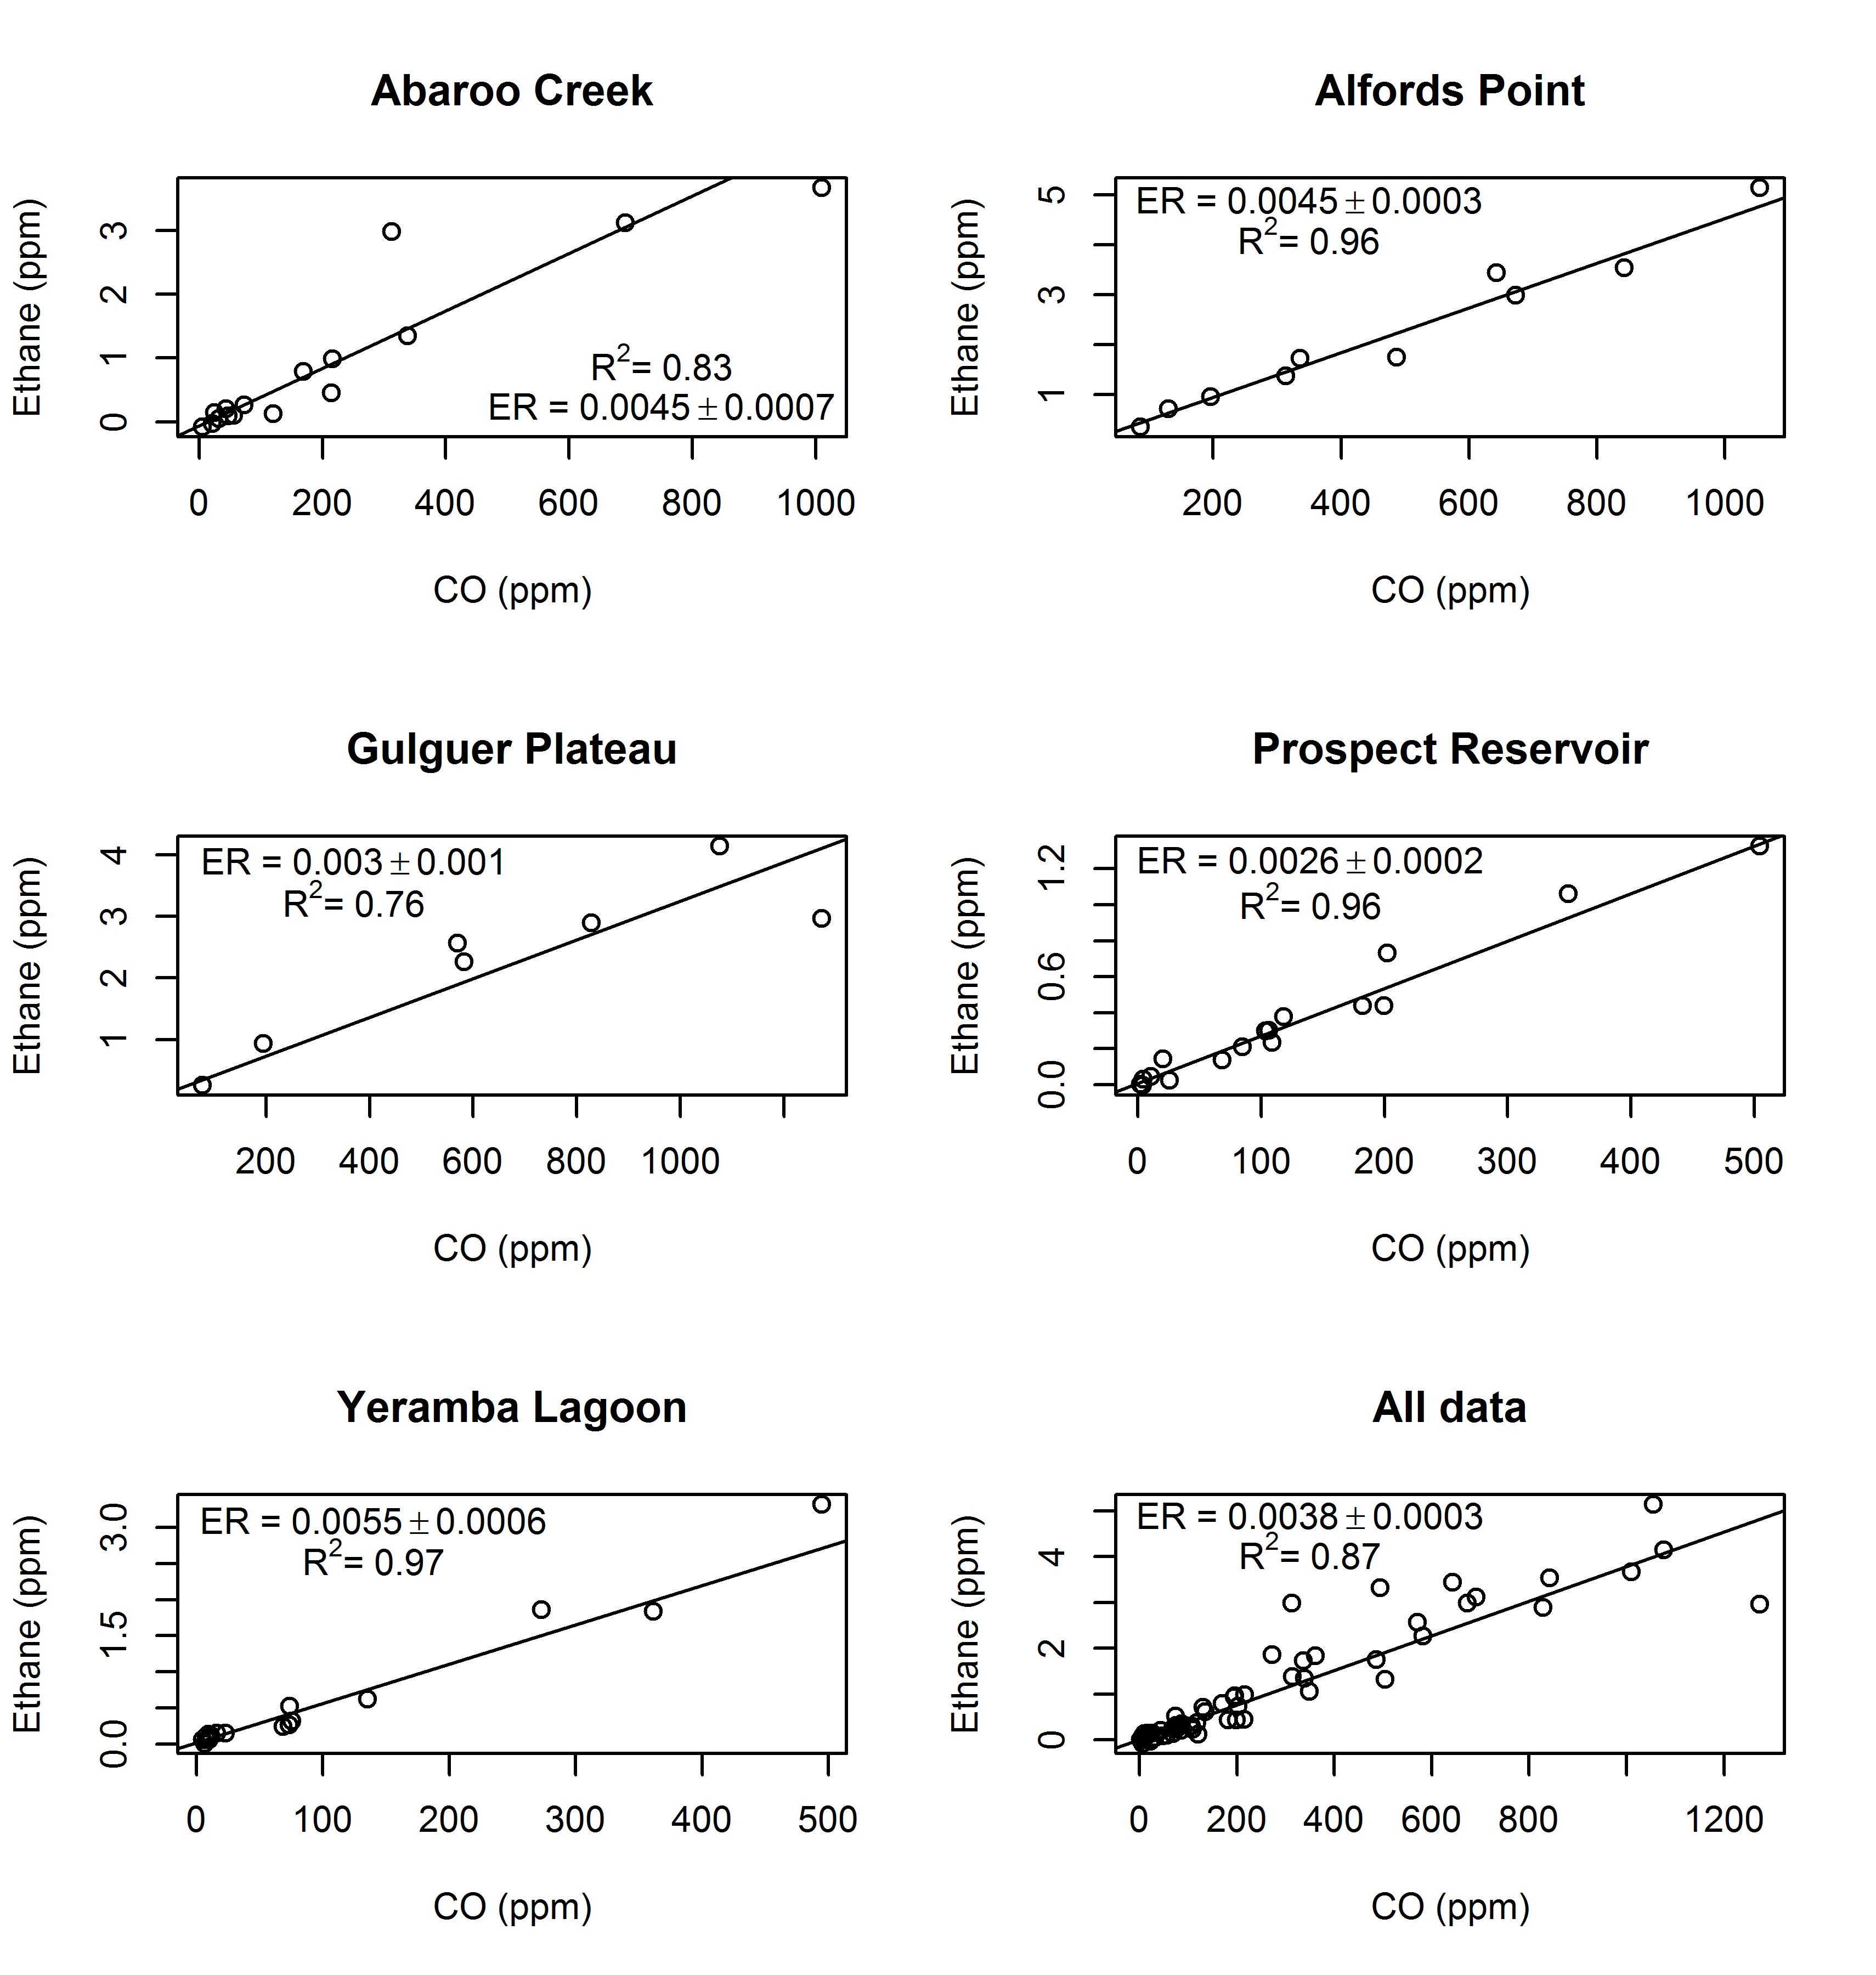
\includegraphics[width=14 cm]{C:/Users/eag873/Documents/GitHub/HRB_paper/supp/supp_figures/Ethane_fire_by_fire.png}
  \caption{Emission ratio of ethane to CO for each individual fire sampled by grab sampling and for all the fires combined. }
  \label{fig:Ethane}
\end{figure}



\section{Additional open-path FTIR results}
All trace gases measured by open-path FTIR at the prescribed fires in Victoria exhibited strong correlations with either CO or CO$_2$. Correlations between the measured species at the Castlemaine fire are shown in Figure~\ref{fig:Castlemaine} as an example. 

\begin{figure}
  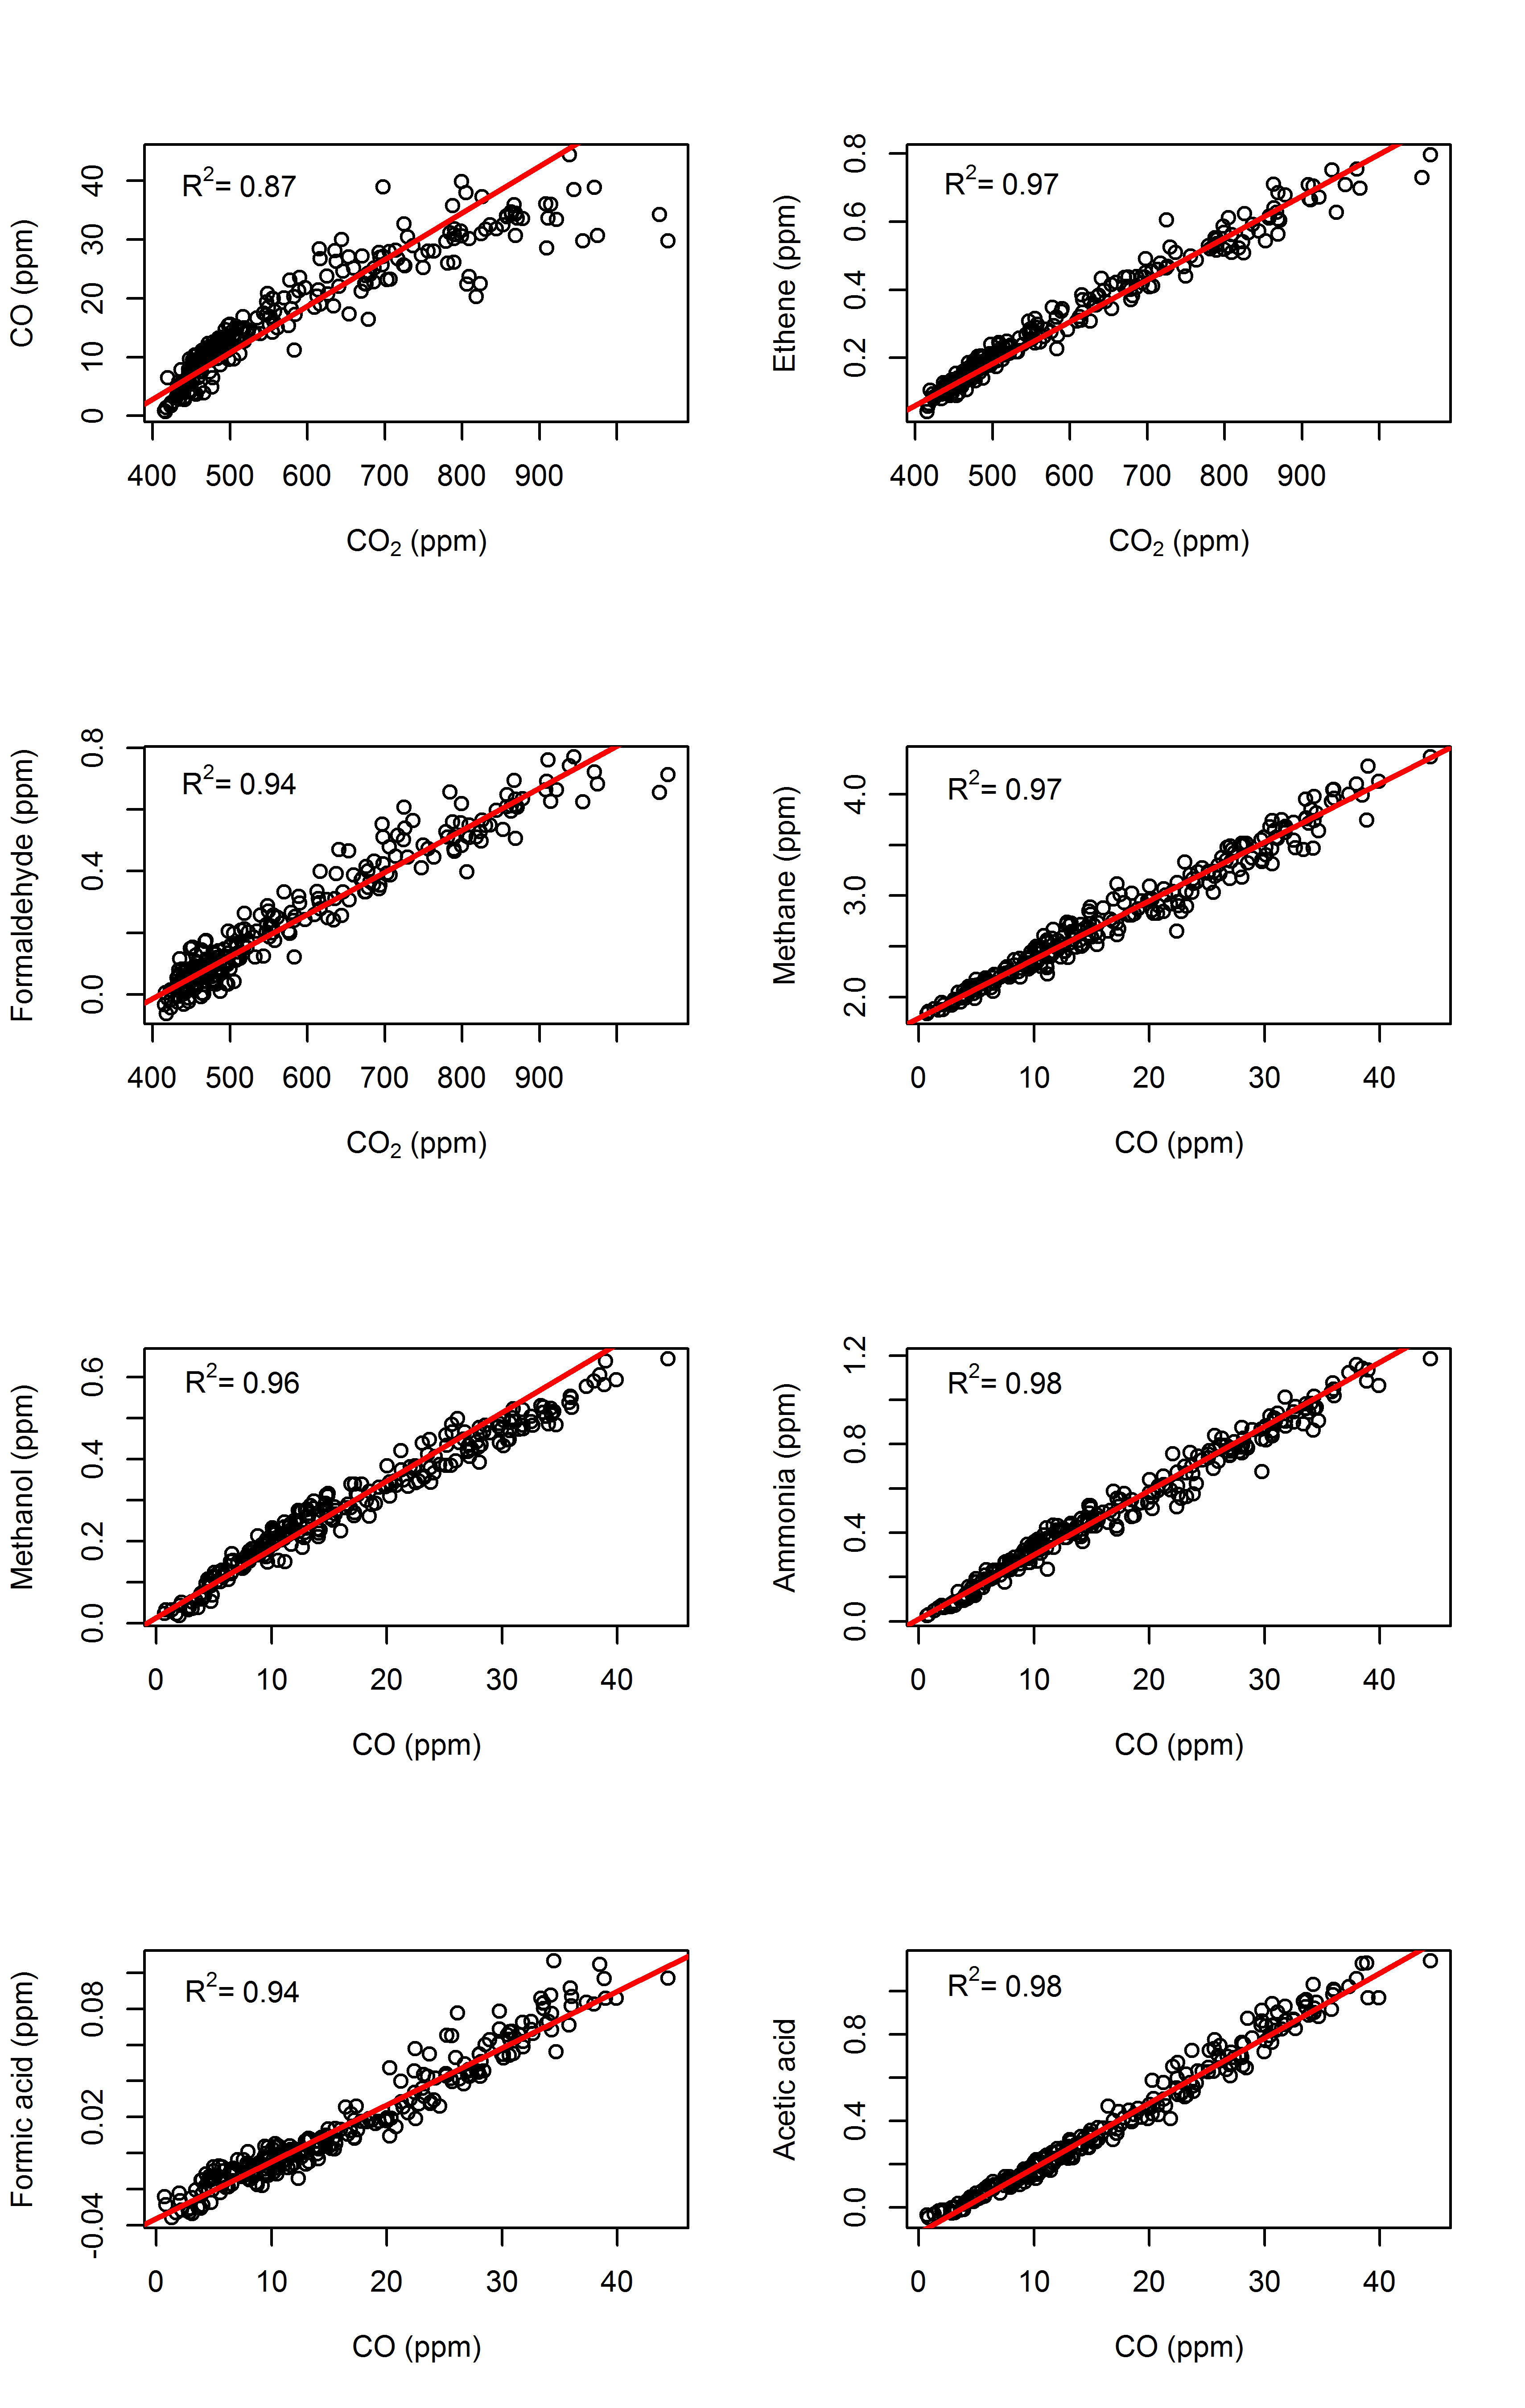
\includegraphics[width=12.5 cm]{C:/Users/eag873/Documents/GitHub/HRB_paper/supp/supp_figures/Castlemaine.png}
  \caption{Correlation plots for open-path FTIR measurements at the Castlemaine, VIC fire.}
  \label{fig:Castlemaine}
\end{figure}




\bibliographystyle{copernicus}
\bibliography{C:/Users/eag873/Documents/GitHub/HRB_paper/references}

\end{document}